\section{Capítulo 8 -- Ordenação}

No Capítulo 7 você viu que a busca binária encontra um valor entre um bilhão em 30 comparações, desde que o vetor esteja \textbf{ordenado}. Ordenar dados é uma das tarefas mais comuns da computação: listas de alunos em ordem alfabética, produtos do mais barato ao mais caro, mensagens da mais recente à mais antiga. Também é um dos melhores lugares para aprender a projetar algoritmos, porque o mesmo problema tem soluções muito diferentes. Neste capítulo você vai estudar seis delas: três simples, de custo $O(n^2)$, e três eficientes, de custo $O(n \log n)$. No caminho, vai construir o \textit{heap}, a estrutura que o Capítulo 6 usou dentro da fila de prioridade.

\subsection{8.1 O problema da ordenação}

Ordenar é rearranjar os elementos de um vetor para que fiquem em ordem crescente (ou decrescente) segundo algum critério. Todos os algoritmos deste capítulo são \textbf{baseados em comparações}: a única coisa que fazem com os elementos é perguntar ``este é menor que aquele?'' e trocá-los de lugar. Por isso, servem para qualquer tipo que saiba se comparar, de números a nomes e datas.

Além do tempo, três características ajudam a escolher um algoritmo:

\begin{itemize}
  \item \textbf{No lugar} (\textit{in-place}): o algoritmo usa apenas uma quantidade constante de memória extra, além do próprio vetor.
  \item \textbf{Estável}: elementos com a mesma chave continuam na ordem em que estavam. Se uma turma já está em ordem alfabética e você a ordena por nota com um algoritmo estável, os alunos com a mesma nota continuam em ordem alfabética.
  \item \textbf{Adaptativo}: o algoritmo trabalha menos quando o vetor já está quase ordenado.
\end{itemize}

Todos os exemplos usam o mesmo vetor de oito números, \texttt{\{29, 10, 14, 37, 13, 5, 41, 22\}}, e a função \texttt{swap} do C++, que troca o conteúdo de duas variáveis.

\subsection{8.2 Ordenação por bolha (\textit{bubble sort})}

A ordenação por bolha percorre o vetor comparando cada par de vizinhos e trocando os dois sempre que estiverem fora de ordem. Ao fim da primeira passada, o maior elemento foi empurrado, troca a troca, até a última posição, como uma bolha que sobe até a superfície. A segunda passada leva o segundo maior para a penúltima posição, e assim por diante.

\begin{center}
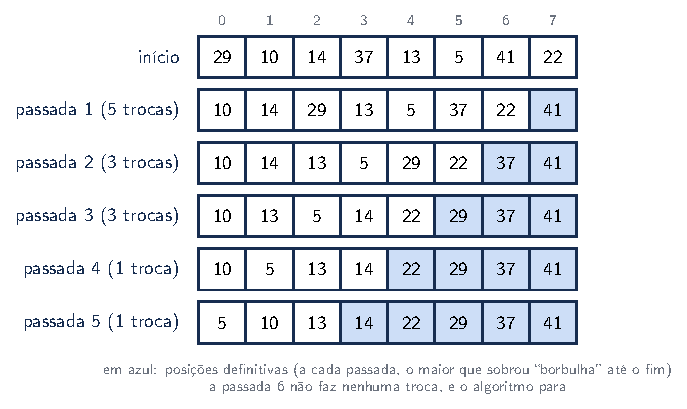
\includegraphics[width=0.85\linewidth,keepaspectratio]{imagens/capitulo-08_bolha.pdf}
\end{center}

\begin{codigo}
\begin{Verbatim}[breaklines=true, breaksymbolleft={}, fontsize=\footnotesize]
// trecho
void bolha(vector<int> &v) {
    int n = static_cast<int>(v.size());
    for (int passada = 0; passada < n - 1; passada++) {
        bool trocou = false;
        // os últimos "passada" elementos já estão no lugar
        for (int i = 0; i < n - 1 - passada; i++) {
            if (v[i] > v[i + 1]) {
                swap(v[i], v[i + 1]);
                trocou = true;
            }
        }
        if (!trocou) return;   // nenhuma troca: já está ordenado
    }
}
\end{Verbatim}
\end{codigo}

A variável \texttt{trocou} é o que torna a bolha adaptativa: se uma passada inteira não fizer nenhuma troca, o vetor já está ordenado e o algoritmo para. Em um vetor já ordenado, basta uma passada, $O(n)$. No pior caso, o vetor em ordem inversa, são $n - 1$ passadas com cerca de $n^2/2$ comparações e trocas: $O(n^2)$. A bolha é estável, porque só troca vizinhos estritamente fora de ordem, e funciona no lugar.

\subsection{8.3 Ordenação por seleção (\textit{selection sort})}

A ordenação por seleção faz o que muita gente faria à mão: procura o menor elemento e o coloca na primeira posição; depois procura o menor entre os que sobraram e o coloca na segunda, e assim por diante.

\begin{codigo}
\begin{Verbatim}[breaklines=true, breaksymbolleft={}, fontsize=\footnotesize]
// trecho
void selecao(vector<int> &v) {
    int n = static_cast<int>(v.size());
    for (int i = 0; i < n - 1; i++) {
        int menor = i;
        for (int j = i + 1; j < n; j++) {  // o menor do resto
            if (v[j] < v[menor]) menor = j;
        }
        swap(v[i], v[menor]);              // uma troca só
    }
}
\end{Verbatim}
\end{codigo}

A seleção sempre faz cerca de $n^2/2$ comparações, mesmo que o vetor já esteja ordenado: ela não é adaptativa, e é $O(n^2)$ em todos os casos. Sua vantagem é fazer no máximo $n - 1$ trocas, o que importa quando mover um elemento custa muito mais que compará-lo. Ela não é estável: a troca pode levar um elemento para depois de outro igual a ele.

\subsection{8.4 Ordenação por inserção (\textit{insertion sort})}

A ordenação por inserção é o jeito como se arruma uma mão de cartas: as cartas da esquerda já estão em ordem, e cada nova carta é encaixada no lugar certo entre elas. No vetor, a parte ordenada começa com um único elemento e cresce uma posição a cada passo. Para abrir espaço para o novo elemento, os maiores que ele são deslocados uma posição para a direita.

\begin{center}
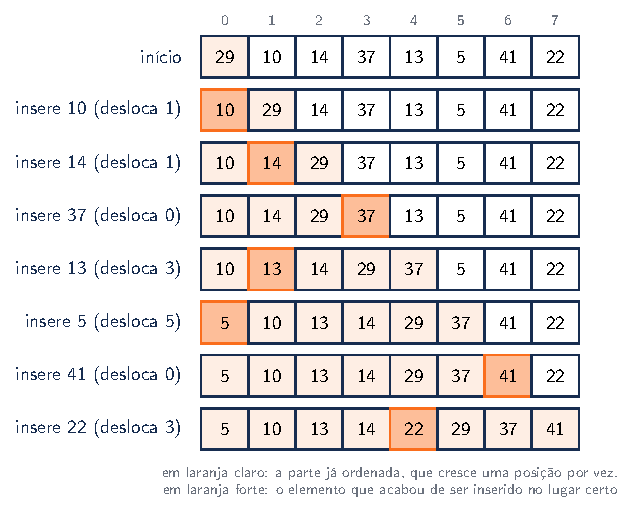
\includegraphics[width=0.85\linewidth,keepaspectratio]{imagens/capitulo-08_insercao.pdf}
\end{center}

\begin{codigo}
\begin{Verbatim}[breaklines=true, breaksymbolleft={}, fontsize=\footnotesize]
// trecho
void insercao(vector<int> &v) {
    int n = static_cast<int>(v.size());
    for (int i = 1; i < n; i++) {
        int chave = v[i];        // o próximo a ser inserido
        int j = i - 1;
        while (j >= 0 && v[j] > chave) {
            v[j + 1] = v[j];     // desloca o maior à direita
            j--;
        }
        v[j + 1] = chave;        // encaixa no espaço aberto
    }
}
\end{Verbatim}
\end{codigo}

O laço \texttt{while} para assim que encontra um elemento menor ou igual à chave. Em um vetor já ordenado, ele para logo na primeira comparação, e a inserção inteira custa $O(n)$; em um vetor quase ordenado, faz poucos deslocamentos. No pior caso, em ordem inversa, cada elemento percorre toda a parte ordenada: $O(n^2)$. A inserção é estável, porque o \texttt{>} nunca passa uma chave para antes de outra igual, e funciona no lugar.

O programa completo ordena o vetor de exemplo com os três algoritmos:

\begin{codigo}
\begin{Verbatim}[breaklines=true, breaksymbolleft={}, fontsize=\footnotesize]
#include <vector>
#include <utility>   // swap

void bolha(vector<int> &v) {
    int n = static_cast<int>(v.size());
    for (int passada = 0; passada < n - 1; passada++) {
        bool trocou = false;
        for (int i = 0; i < n - 1 - passada; i++) {
            if (v[i] > v[i + 1]) {
                swap(v[i], v[i + 1]);
                trocou = true;
            }
        }
        if (!trocou) return;
    }
}

void selecao(vector<int> &v) {
    int n = static_cast<int>(v.size());
    for (int i = 0; i < n - 1; i++) {
        int menor = i;
        for (int j = i + 1; j < n; j++) {
            if (v[j] < v[menor]) menor = j;
        }
        swap(v[i], v[menor]);
    }
}

void insercao(vector<int> &v) {
    int n = static_cast<int>(v.size());
    for (int i = 1; i < n; i++) {
        int chave = v[i];
        int j = i - 1;
        while (j >= 0 && v[j] > chave) {
            v[j + 1] = v[j];
            j--;
        }
        v[j + 1] = chave;
    }
}

void mostrar(const vector<int> &v) {
    for (int x : v) cout << x << " ";
    cout << endl;
}

int main() {
    const vector<int> exemplo = {29, 10, 14, 37, 13, 5, 41, 22};
    vector<int> a = exemplo, b = exemplo, c = exemplo;
    bolha(a);
    selecao(b);
    insercao(c);
    mostrar(a);   // 5 10 13 14 22 29 37 41
    mostrar(b);   // 5 10 13 14 22 29 37 41
    mostrar(c);   // 5 10 13 14 22 29 37 41
}
\end{Verbatim}
\end{codigo}

Os três são $O(n^2)$ no pior caso, mas se comportam de forma bem diferente conforme a entrada. Esta tabela mostra quantas comparações e quantas trocas (ou deslocamentos, na inserção) cada um faz em um vetor de 1.000 elementos, no formato ``comparações / trocas'':

\begin{center}
\begin{tabular}{@{}p{0.24\linewidth}p{0.3\linewidth}p{0.32\linewidth}@{}}
\toprule
\rowcolor{headergray}
\tblheader{Algoritmo} & \tblheader{Já ordenado} & \tblheader{Em ordem inversa} \\
\midrule
bolha & 999 / 0 & 499.500 / 499.500 \\
\rowcolor{rowgray} seleção & 499.500 / 999 & 499.500 / 999 \\
inserção & 999 / 0 & 499.500 / 499.500 \\
\bottomrule
\end{tabular}
\end{center}

Na prática, a inserção é a melhor dos três: é simples, estável, adaptativa e muito rápida em vetores pequenos ou quase ordenados. Por isso, ela aparece dentro dos algoritmos de ordenação das bibliotecas, como você verá na Seção 8.8.

\subsection{8.5 Ordenação por intercalação (\textit{merge sort})}

Para fugir do $O(n^2)$, é preciso parar de comparar quase todos os pares. A ordenação por intercalação usa a estratégia \textbf{dividir para conquistar}, a mesma ideia de reduzir um problema a problemas menores que você viu na recursão:

\begin{enumerate}
  \item \textbf{Dividir}: separe o vetor em duas metades.
  \item \textbf{Conquistar}: ordene cada metade, recursivamente. Um vetor com zero ou um elemento já está ordenado.
  \item \textbf{Combinar}: \textbf{intercale} as duas metades ordenadas em um único vetor ordenado.
\end{enumerate}

\begin{center}
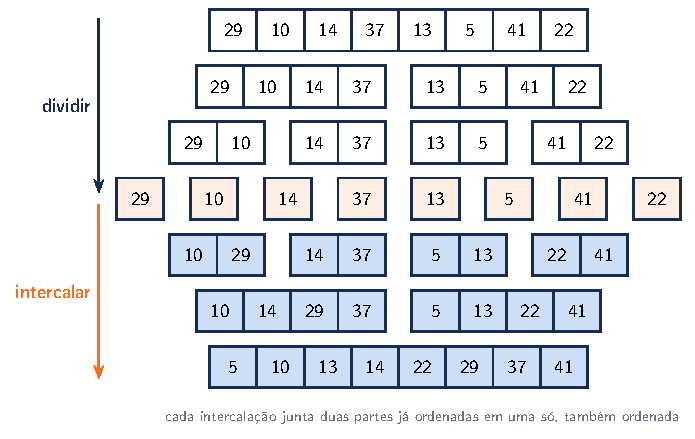
\includegraphics[width=0.85\linewidth,keepaspectratio]{imagens/capitulo-08_intercalacao.pdf}
\end{center}

Todo o trabalho está na intercalação. Como as duas metades já estão ordenadas, o menor de todos só pode ser o primeiro de uma delas. Basta comparar os primeiros de cada metade, copiar o menor para um vetor auxiliar e avançar naquela metade, até uma delas acabar; o que sobrar da outra já está em ordem e é copiado no fim.

\begin{codigo}
\begin{Verbatim}[breaklines=true, breaksymbolleft={}, fontsize=\footnotesize]
// trecho
// junta v[ini..meio] e v[meio+1..fim], já ordenados, em um só
void intercalar(vector<int> &v, int ini, int meio, int fim) {
    vector<int> aux;
    aux.reserve(fim - ini + 1);
    int i = ini, j = meio + 1;
    while (i <= meio && j <= fim) {
        if (v[i] <= v[j]) {      // empate: a esquerda primeiro
            aux.push_back(v[i++]);
        } else {
            aux.push_back(v[j++]);
        }
    }
    while (i <= meio) aux.push_back(v[i++]);  // sobras: esquerda
    while (j <= fim) aux.push_back(v[j++]);   // sobras: direita
    for (int k = 0; k < static_cast<int>(aux.size()); k++) {
        v[ini + k] = aux[k];                  // copia de volta
    }
}

void mergeSort(vector<int> &v, int ini, int fim) {
    if (ini >= fim) return;      // 0 ou 1 elemento: já ordenado
    int meio = ini + (fim - ini) / 2;
    mergeSort(v, ini, meio);
    mergeSort(v, meio + 1, fim);
    intercalar(v, ini, meio, fim);
}
\end{Verbatim}
\end{codigo}

O \texttt{v[i++]} usa o valor de \texttt{v[i]} e só depois avança o \texttt{i}. O \texttt{<=} na comparação faz o \textit{merge sort} ser estável: em caso de empate, o elemento da metade esquerda, que vinha antes, é copiado primeiro.

Para calcular o custo, olhe a figura por níveis. Intercalar todos os pedaços de um mesmo nível custa $O(n)$, porque cada elemento é copiado uma vez. E, como o vetor é dividido ao meio a cada nível, existem $\log_2 n$ níveis (3, para 8 elementos). O total é $O(n \log n)$, \textbf{em qualquer caso}: o \textit{merge sort} não depende da ordem da entrada. O preço é a memória: o vetor auxiliar ocupa $O(n)$, então ele não funciona no lugar.

\subsection{8.6 Ordenação rápida (\textit{quicksort})}

O \textit{quicksort} também divide para conquistar, mas faz o trabalho pesado \textbf{antes} da recursão, e não depois. Ele escolhe um elemento, o \textbf{pivô}, e \textbf{particiona} o vetor: os menores que o pivô vão para a esquerda, os maiores para a direita, e o pivô fica entre os dois grupos, que é exatamente a sua posição final. Depois, basta ordenar cada grupo recursivamente. Não há nada para combinar.

\begin{center}
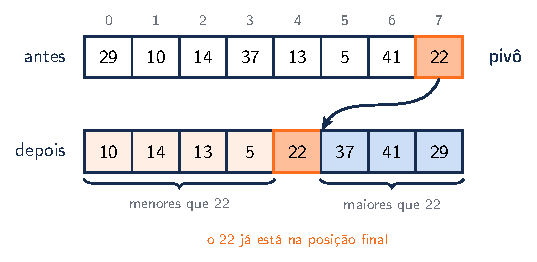
\includegraphics[width=0.75\linewidth,keepaspectratio]{imagens/capitulo-08_particao.pdf}
\end{center}

A partição abaixo usa o último elemento como pivô. A variável \texttt{i} marca o fim da região dos menores; cada elemento menor que o pivô encontrado por \texttt{j} é trocado para dentro dessa região, que cresce uma posição. No final, o pivô é trocado para logo depois dela.

\begin{codigo}
\begin{Verbatim}[breaklines=true, breaksymbolleft={}, fontsize=\footnotesize]
// trecho
// põe o pivô (o último) na posição final e devolve essa posição
int particionar(vector<int> &v, int ini, int fim) {
    int pivo = v[fim];
    int i = ini - 1;          // fim da região dos menores
    for (int j = ini; j < fim; j++) {
        if (v[j] < pivo) {
            i++;
            swap(v[i], v[j]); // entra na região dos menores
        }
    }
    swap(v[i + 1], v[fim]);   // pivô logo após os menores
    return i + 1;
}

void quickSort(vector<int> &v, int ini, int fim) {
    if (ini >= fim) return;
    int p = particionar(v, ini, fim);
    quickSort(v, ini, p - 1); // o pivô já está no lugar
    quickSort(v, p + 1, fim);
}
\end{Verbatim}
\end{codigo}

O custo depende de quão bem o pivô divide o vetor. Quando os dois grupos têm tamanhos parecidos, a recursão tem cerca de $\log_2 n$ níveis, cada um com $O(n)$ comparações, e o \textit{quicksort} é $O(n \log n)$. Na prática, ele costuma ser o mais rápido de todos, porque faz poucas trocas, não copia o vetor e percorre a memória em sequência.

\begin{destaque}{O pior caso do quicksort}
Se o pivô for sempre o maior ou o menor elemento, um dos grupos fica vazio e o outro tem $n - 1$ elementos. A recursão passa a ter $n$ níveis, e o custo vira $O(n^2)$. Com o último elemento como pivô, isso acontece justamente com um vetor \textbf{já ordenado}, uma entrada muito comum. Além de lento, o algoritmo pode estourar a pilha de execução com milhares de chamadas recursivas aninhadas. A solução é escolher melhor o pivô: o elemento do meio, um elemento sorteado ou a mediana entre o primeiro, o do meio e o último. Na partição acima, basta trocar o escolhido com o último antes de começar:

\begin{codigo}
\begin{Verbatim}[breaklines=true, breaksymbolleft={}, fontsize=\footnotesize]
// trecho
int meio = ini + (fim - ini) / 2;
swap(v[meio], v[fim]);   // o do meio passa a ser o pivô
\end{Verbatim}
\end{codigo}
\end{destaque}

O \textit{quicksort} funciona no lugar, usando só a pilha da recursão, $O(\log n)$ em média. Ele não é estável, porque as trocas da partição podem levar um elemento para longe, passando por cima de outros iguais a ele.

O programa completo testa os dois algoritmos no vetor de exemplo e em um vetor de 100 mil números pseudoaleatórios:

\begin{codigo}
\begin{Verbatim}[breaklines=true, breaksymbolleft={}, fontsize=\footnotesize]
#include <vector>
#include <utility>     // swap
#include <algorithm>   // is_sorted

void intercalar(vector<int> &v, int ini, int meio, int fim) {
    vector<int> aux;
    aux.reserve(fim - ini + 1);
    int i = ini, j = meio + 1;
    while (i <= meio && j <= fim) {
        if (v[i] <= v[j]) {
            aux.push_back(v[i++]);
        } else {
            aux.push_back(v[j++]);
        }
    }
    while (i <= meio) aux.push_back(v[i++]);
    while (j <= fim) aux.push_back(v[j++]);
    for (int k = 0; k < static_cast<int>(aux.size()); k++) {
        v[ini + k] = aux[k];
    }
}

void mergeSort(vector<int> &v, int ini, int fim) {
    if (ini >= fim) return;
    int meio = ini + (fim - ini) / 2;
    mergeSort(v, ini, meio);
    mergeSort(v, meio + 1, fim);
    intercalar(v, ini, meio, fim);
}

int particionar(vector<int> &v, int ini, int fim) {
    int meio = ini + (fim - ini) / 2;
    swap(v[meio], v[fim]);    // o do meio passa a ser o pivô
    int pivo = v[fim];
    int i = ini - 1;
    for (int j = ini; j < fim; j++) {
        if (v[j] < pivo) {
            i++;
            swap(v[i], v[j]);
        }
    }
    swap(v[i + 1], v[fim]);
    return i + 1;
}

void quickSort(vector<int> &v, int ini, int fim) {
    if (ini >= fim) return;
    int p = particionar(v, ini, fim);
    quickSort(v, ini, p - 1);
    quickSort(v, p + 1, fim);
}

int main() {
    vector<int> a = {29, 10, 14, 37, 13, 5, 41, 22};
    vector<int> b = a;
    mergeSort(a, 0, static_cast<int>(a.size()) - 1);
    quickSort(b, 0, static_cast<int>(b.size()) - 1);
    for (int x : a) cout << x << " ";
    cout << endl;             // 5 10 13 14 22 29 37 41

    vector<int> grande(100000);
    unsigned int semente = 42;
    for (int &x : grande) {   // gerador congruencial simples
        semente = semente * 1103515245u + 12345u;
        x = static_cast<int>(semente % 1000000);
    }
    vector<int> c = grande;
    int ultimo = static_cast<int>(grande.size()) - 1;
    mergeSort(grande, 0, ultimo);
    quickSort(c, 0, ultimo);
    cout << boolalpha << is_sorted(grande.begin(), grande.end())
         << " " << (grande == c) << endl;   // true true
}
\end{Verbatim}
\end{codigo}

A função \texttt{is\_sorted}, da biblioteca \texttt{<algorithm>}, confere se um vetor está em ordem, e \texttt{grande == c} compara os dois vetores posição por posição. Testar um algoritmo de ordenação com muitos dados gerados automaticamente encontra erros que um exemplo de oito números não mostraria; o Capítulo 11 volta a esse assunto.

\subsection{8.7 Heap e heapsort}

Um \textbf{heap} (máximo) é uma árvore binária com duas propriedades:

\begin{itemize}
  \item é \textbf{completa}: todos os níveis estão cheios, menos talvez o último, que é preenchido da esquerda para a direita;
  \item cada nó é \textbf{maior ou igual a seus filhos}. Por isso, o maior de todos está sempre na raiz.
\end{itemize}

Diferente da árvore binária de busca do Capítulo 5, o heap não diz nada sobre a ordem entre irmãos; ele só garante que cada pai vence os filhos. E, por ser completo, ele cabe em um vetor sem nenhum ponteiro: basta guardar os nós nível por nível, da esquerda para a direita.

\begin{center}
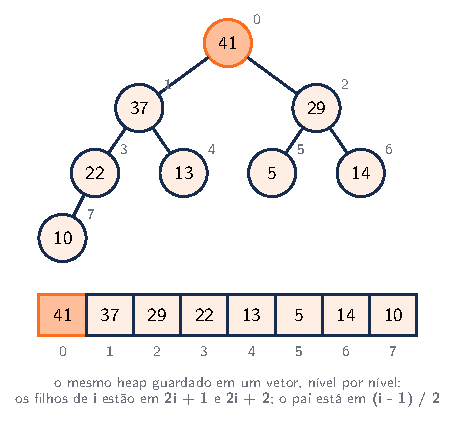
\includegraphics[width=0.65\linewidth,keepaspectratio]{imagens/capitulo-08_heap.pdf}
\end{center}

A operação central do heap é \textbf{descer}: quando um nó é menor que algum filho, ele troca de lugar com o maior dos filhos e continua descendo até ficar maior que os dois, ou chegar a uma folha. Como a altura de uma árvore completa é $\log_2 n$, descer custa $O(\log n)$.

O \textbf{heapsort} usa o heap em duas etapas:

\begin{enumerate}
  \item \textbf{Montar o heap}: faça descer cada nó que tem filhos, do último até a raiz. Ao final, o vetor de exemplo vira o heap da figura.
  \item \textbf{Ordenar}: o maior está na posição 0. Troque-o com o último elemento do heap, que passa a ter uma posição a menos, e faça a nova raiz descer para consertar o heap. Repita até sobrar um elemento. Os maiores vão sendo guardados no fim do vetor, do maior para o menor.
\end{enumerate}

\begin{codigo}
\begin{Verbatim}[breaklines=true, breaksymbolleft={}, fontsize=\footnotesize]
// trecho
// faz v[i] descer até o lugar certo em um heap de n elementos
void descer(vector<int> &v, int i, int n) {
    while (true) {
        int maior = i;
        int esq = 2 * i + 1, dir = 2 * i + 2;
        if (esq < n && v[esq] > v[maior]) maior = esq;
        if (dir < n && v[dir] > v[maior]) maior = dir;
        if (maior == i) return;   // já é maior que os filhos
        swap(v[i], v[maior]);
        i = maior;
    }
}

void heapSort(vector<int> &v) {
    int n = static_cast<int>(v.size());
    for (int i = n / 2 - 1; i >= 0; i--) {  // 1. monta o heap
        descer(v, i, n);
    }
    for (int fim = n - 1; fim > 0; fim--) { // 2. ordena
        swap(v[0], v[fim]);         // o maior vai para o fim
        descer(v, 0, fim);          // conserta o que sobrou
    }
}
\end{Verbatim}
\end{codigo}

Os nós com filhos são os de índice $0$ a $n/2 - 1$; os outros são folhas, que já são heaps de um elemento. Montar o heap custa $O(n)$ (a conta é mais sutil do que parece, porque a maioria dos nós está perto das folhas e desce pouco), e cada uma das $n - 1$ retiradas custa $O(\log n)$. O \textit{heapsort} é $O(n \log n)$ em \textbf{qualquer caso}, como o \textit{merge sort}, e funciona no lugar, como o \textit{quicksort}. Ele não é estável.

\subsubsection{A fila de prioridade}

O heap também é a estrutura por trás da \texttt{priority\_queue} usada pelo Dijkstra e pelo Prim no Capítulo 6. Retirar o maior é o mesmo movimento do \textit{heapsort}: o último elemento vai para a raiz e desce. Inserir é o movimento contrário: o novo elemento entra no fim do vetor e \textbf{sobe}, trocando de lugar com o pai enquanto for maior que ele. As duas operações custam $O(\log n)$.

\begin{codigo}
\begin{Verbatim}[breaklines=true, breaksymbolleft={}, fontsize=\footnotesize]
#include <vector>
#include <utility>   // swap

void descer(vector<int> &v, int i, int n) {
    while (true) {
        int maior = i;
        int esq = 2 * i + 1, dir = 2 * i + 2;
        if (esq < n && v[esq] > v[maior]) maior = esq;
        if (dir < n && v[dir] > v[maior]) maior = dir;
        if (maior == i) return;
        swap(v[i], v[maior]);
        i = maior;
    }
}

void heapSort(vector<int> &v) {
    int n = static_cast<int>(v.size());
    for (int i = n / 2 - 1; i >= 0; i--) {
        descer(v, i, n);
    }
    for (int fim = n - 1; fim > 0; fim--) {
        swap(v[0], v[fim]);
        descer(v, 0, fim);
    }
}

class FilaPrioridade {
private:
    vector<int> dados;   // um heap máximo

public:
    bool vazia() const { return dados.empty(); }

    void inserir(int valor) {
        dados.push_back(valor);          // entra no fim...
        int i = static_cast<int>(dados.size()) - 1;
        while (i > 0 && dados[(i - 1) / 2] < dados[i]) {
            swap(dados[i], dados[(i - 1) / 2]);  // ...e sobe
            i = (i - 1) / 2;
        }
    }

    int remover() {                      // tira o maior
        int maior = dados[0];
        dados[0] = dados.back();         // o último vai à raiz...
        dados.pop_back();
        int n = static_cast<int>(dados.size());
        descer(dados, 0, n);             // ...e desce
        return maior;
    }
};

int main() {
    vector<int> v = {29, 10, 14, 37, 13, 5, 41, 22};
    heapSort(v);
    for (int x : v) cout << x << " ";
    cout << endl;                // 5 10 13 14 22 29 37 41

    FilaPrioridade fila;
    for (int x : {29, 10, 14, 37, 13}) fila.inserir(x);
    while (!fila.vazia()) cout << fila.remover() << " ";
    cout << endl;                // 37 29 14 13 10
}
\end{Verbatim}
\end{codigo}

\subsection{8.8 Comparando os algoritmos}

\begin{center}
\begin{tabular}{@{}p{0.2\linewidth}p{0.17\linewidth}p{0.17\linewidth}p{0.14\linewidth}p{0.1\linewidth}@{}}
\toprule
\rowcolor{headergray}
\tblheader{Algoritmo} & \tblheader{Médio} & \tblheader{Pior} & \tblheader{Memória} & \tblheader{Estável} \\
\midrule
bolha & $O(n^2)$ & $O(n^2)$ & $O(1)$ & sim \\
\rowcolor{rowgray} seleção & $O(n^2)$ & $O(n^2)$ & $O(1)$ & não \\
inserção & $O(n^2)$ & $O(n^2)$ & $O(1)$ & sim \\
\rowcolor{rowgray} \textit{merge sort} & $O(n \log n)$ & $O(n \log n)$ & $O(n)$ & sim \\
\textit{quicksort} & $O(n \log n)$ & $O(n^2)$ & $O(\log n)$ & não \\
\rowcolor{rowgray} \textit{heapsort} & $O(n \log n)$ & $O(n \log n)$ & $O(1)$ & não \\
\bottomrule
\end{tabular}
\end{center}

Nenhum é o melhor em tudo. O \textit{merge sort} é previsível e estável, mas gasta memória; o \textit{quicksort} é o mais rápido na média, mas tem um pior caso ruim; o \textit{heapsort} garante $O(n \log n)$ no lugar, mas costuma ser mais lento que os outros dois na prática. E, em vetores pequenos, de algumas dezenas de elementos, a simples inserção vence todos eles, porque faz pouquíssimo trabalho por passo.

\begin{destaque}{Dá para ordenar mais rápido que $O(n \log n)$?}
Não, se o algoritmo só puder comparar elementos. Um vetor de $n$ elementos pode estar em $n!$ ordens diferentes, e cada comparação, com resposta ``sim'' ou ``não'', no máximo corta pela metade as ordens ainda possíveis. Para separar todas elas são necessárias pelo menos $\log_2 (n!)$ comparações, que é da ordem de $n \log n$: para 1.000 elementos, cerca de 8.500. Algoritmos que não comparam, como a ordenação por contagem (\textit{counting sort}), escapam desse limite, mas só funcionam para chaves especiais, como inteiros em uma faixa pequena.
\end{destaque}

\subsubsection{Ordenação na biblioteca padrão}

No dia a dia, use a \texttt{sort} da biblioteca \texttt{<algorithm>}. Ela é um \textbf{introsort}: começa como um \textit{quicksort}, passa para o \textit{heapsort} se a recursão ficar funda demais (fugindo do pior caso) e termina os pedaços pequenos com a inserção. Quando precisar de estabilidade, use a \texttt{stable\_sort}, que é um \textit{merge sort}.

As duas aceitam um terceiro parâmetro, o \textbf{critério de comparação}: uma função que recebe dois elementos e responde se o primeiro deve vir antes do segundo. Ele pode ser um objeto pronto, como \texttt{greater<>()} para a ordem decrescente, ou uma função anônima (\textit{lambda}), escrita ali mesmo, que você vai estudar no Capítulo 10.

\begin{codigo}
\begin{Verbatim}[breaklines=true, breaksymbolleft={}, fontsize=\footnotesize]
#include <vector>
#include <algorithm>    // sort, stable_sort
#include <functional>   // greater

struct Aluno {
    string nome;
    double nota;
};

int main() {
    vector<int> v = {29, 10, 14, 37, 13, 5, 41, 22};
    sort(v.begin(), v.end());                // crescente
    sort(v.begin(), v.end(), greater<>());   // decrescente
    for (int x : v) cout << x << " ";
    cout << endl;                // 41 37 29 22 14 13 10 5

    vector<Aluno> turma = {{"Davi", 7.5}, {"Ana", 9.0},
                           {"Caio", 7.5}, {"Bia", 9.0}};
    // maior nota primeiro; no empate, mantém a ordem original
    stable_sort(turma.begin(), turma.end(),
                [](const Aluno &a, const Aluno &b) {
                    return a.nota > b.nota;
                });
    for (const Aluno &a : turma) cout << a.nome << " ";
    cout << endl;                // Ana Bia Davi Caio
}
\end{Verbatim}
\end{codigo}

Repare no resultado: Ana e Bia têm 9,0 e aparecem na ordem em que estavam (Ana antes de Bia), e o mesmo acontece com Davi e Caio. Com a \texttt{sort}, que não é estável, a ordem dentro de cada empate poderia ser qualquer uma.

\begin{destaque}{Comparando com Python}
Em Python, \texttt{sorted(lista)} devolve uma nova lista ordenada e \texttt{lista.sort()} ordena a própria lista. Os dois usam o \textbf{Timsort}, uma combinação de \textit{merge sort} e inserção que aproveita os trechos já ordenados da entrada. Ele é estável e $O(n \log n)$. Em vez de um critério de comparação, o Python usa uma \textbf{chave}: o parâmetro \texttt{key} recebe uma função que diz por qual valor cada elemento deve ser ordenado.

\begin{codigo}
\begin{Verbatim}[breaklines=true, breaksymbolleft={}, fontsize=\footnotesize]
numeros = [29, 10, 14, 37, 13, 5, 41, 22]
print(sorted(numeros))          # nova lista, em ordem crescente
numeros.sort(reverse=True)      # ordena a própria lista
print(numeros)                  # [41, 37, 29, 22, 14, 13, 10, 5]

turma = [('Davi', 7.5), ('Ana', 9.0), ('Caio', 7.5), ('Bia', 9.0)]
por_nota = sorted(turma, key=lambda aluno: aluno[1], reverse=True)
print([nome for nome, _ in por_nota])
# ['Ana', 'Bia', 'Davi', 'Caio']

def merge_sort(v):
    if len(v) <= 1:
        return v
    meio = len(v) // 2
    esquerda, direita = merge_sort(v[:meio]), merge_sort(v[meio:])
    resultado = []
    i = j = 0
    while i < len(esquerda) and j < len(direita):
        if esquerda[i] <= direita[j]:
            resultado.append(esquerda[i])
            i += 1
        else:
            resultado.append(direita[j])
            j += 1
    return resultado + esquerda[i:] + direita[j:]

print(merge_sort([29, 10, 14, 37, 13, 5, 41, 22]))
\end{Verbatim}
\end{codigo}

O fatiamento (\texttt{v[:meio]}, \texttt{esquerda[i:]}) deixa o \textit{merge sort} em Python bem curto, mas cada fatia cria uma lista nova. O módulo \texttt{heapq}, visto no Capítulo 6, oferece as operações do heap prontas sobre uma lista comum.
\end{destaque}

\subsection{Erros Comuns}

\begin{itemize}
  \item \textbf{Passar do fim do vetor na bolha.} O laço interno compara \texttt{v[i]} com \texttt{v[i + 1]}, então \texttt{i} precisa parar em \texttt{n - 2}. Com \texttt{i < n}, a última comparação lê uma posição que não existe.
  \item \textbf{Inverter as condições do \texttt{while} da inserção.} Em \texttt{while (v[j] > chave \&\& j >= 0)}, o \texttt{v[-1]} é lido antes de o \texttt{j >= 0} ser testado. A ordem certa é \texttt{j >= 0 \&\& v[j] > chave}: o \texttt{\&\&} para na primeira condição falsa.
  \item \textbf{Esquecer as sobras na intercalação.} Quando uma metade acaba, os elementos restantes da outra precisam ser copiados; sem os dois \texttt{while} finais, eles se perdem.
  \item \textbf{Usar \texttt{<} em vez de \texttt{<=} na intercalação.} O vetor continua ordenado, mas o \textit{merge sort} deixa de ser estável.
  \item \textbf{Usar sempre o último elemento como pivô.} Com dados já ordenados, o \textit{quicksort} vira $O(n^2)$ e pode estourar a pilha.
  \item \textbf{Achar que $O(n^2)$ é sempre pior.} Para vetores pequenos ou quase ordenados, a inserção costuma ser mais rápida que os algoritmos $O(n \log n)$.
  \item \textbf{Usar \texttt{<=} no critério de comparação da \texttt{sort}.} O critério precisa responder \texttt{false} quando os dois elementos são iguais. Com \texttt{<=}, o comportamento é indefinido, e o programa pode até travar.
  \item \textbf{Ordenar uma cópia sem perceber.} Se a função de ordenação recebe o vetor por valor, como em \texttt{vector<int> v}, ela ordena uma cópia, e o original continua igual. Use referência: \texttt{vector<int> \&v}.
\end{itemize}
